\begin{illustration}{Kommunikations-Modell unserer Broadcasting-Anwendung}

\tikzset{
  rect/.style={draw,fill=green!15,minimum height=0.8cm,rectangle},
  box/.style={
    draw=blue!50!white,
    line width=1pt,
    dash pattern=on 1pt off 4pt on 6pt off 4pt,
    inner sep=4mm, rectangle, rounded corners
  },
}

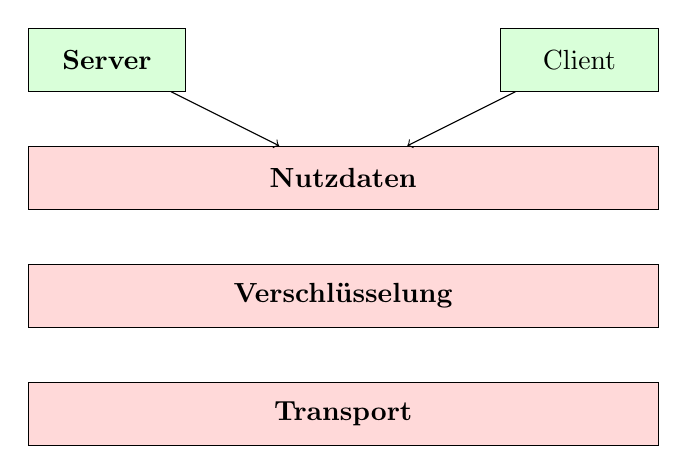
\begin{tikzpicture}[auto,node distance=1.5cm]

\node[rect,minimum width=2cm](server) {\textbf{Server}};
\node[rect,minimum width=2cm,xshift=4.5cm,right of=server](client) {Client};

\node[rect,minimum width=8cm,fill=red!15,below of=server,xshift=3cm,](data)
    {\textbf{Nutzdaten}};

\node[rect,minimum width=8cm,fill=red!15,below of=data](encryption)
    {\textbf{Verschlüsselung}};

\node[rect,minimum width=8cm,fill=red!15,below of=encryption](transport)
    {\textbf{Transport}};

\path[->]
  (server) edge node {} (data)
  (client) edge node {} (data)
 
  ;

\end{tikzpicture}

\end{illustration}